\documentclass[tikz]{standalone}


%\usetikzlibrary{scopes}
\usetikzlibrary{shapes, shapes.geometric, shapes.misc, shapes.arrows}
%\usetikzlibrary{3d, perspective}
\usetikzlibrary{arrows, arrows.meta}
\usetikzlibrary{angles, math, calc, matrix}
\usetikzlibrary {positioning}
%\usetikzlibrary{fadings, shadows, shadings}
\usetikzlibrary{decorations.pathreplacing, decorations.markings, decorations.text, calligraphy}
%\usetikzlibrary{circuits.ee.IEC}

\begin{document}

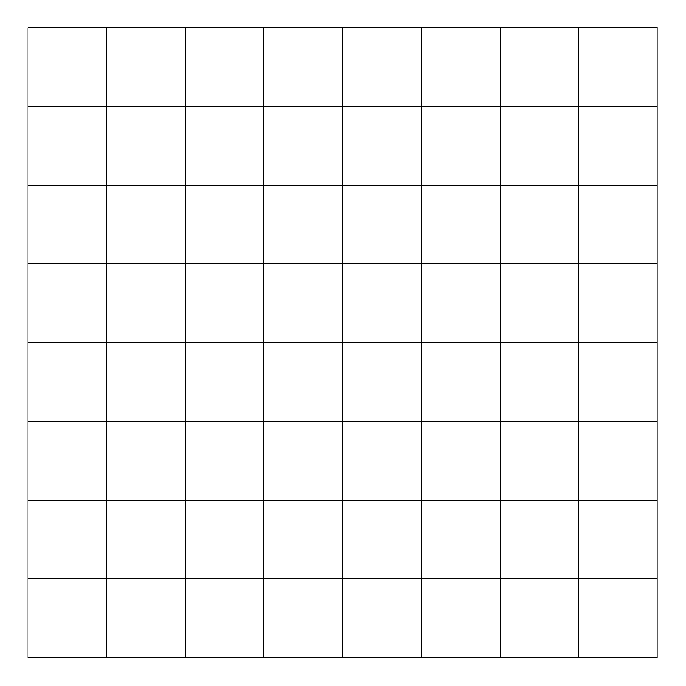
\begin{tikzpicture}
    \clip (-4,-0) rectangle (4,8);
    \draw (-4,-0) grid (4,8);


    

    
\end{tikzpicture}

\end{document}